\documentclass[a4paper,10pt]{article}
\usepackage[utf8]{inputenc}
\usepackage[final]{pdfpages}
\usepackage{fancyref}
\usepackage{caption}

\newcommand{\fw}{\linewidth}

\title{Math 660: Problem Set 4}
\author{Matthew Grasinger}

\begin{document}
  \maketitle
  \tableofcontents

	\section{C1: Crank-Nicolson Scheme, Hyperbolic equations} \label{sec:c1}
	
	In the figures that follow this brief discussion, the Crank-Nicolson discrete approximation using the Thomas algorithm applied to the hyperbolic equation, $u_t + u_x = 0$, is plotted against the exact solution for $h = \frac{1}{10}, \frac{1}{20}$ and $\frac{1}{40}$.
	The relative $L_\infty$ errors at $t = 1.0$ were $0.271$, $0.104$, and $0.045$ for the $h = \frac{1}{10}, \frac{1}{20}$ and $\frac{1}{40}$ approximations, respectively.
	The error was primarily due to truncation error in the Crank-Nicolson scheme, as opposed to round off error in solution of the tridiagonal linear system of equations using the Thomas algorithm.
	This conclusion was made by comparing the solution using the Thomas algorithm to another solution using Gaussian elimination with partial pivoting.
	The difference between the Thomas algorithm solution and the Gaussian elimination with partial pivoting solutions were negligible (order of $10^{-15}$).
	As expected, the error of the Crank-Nicolson scheme decreases with decreasing grid spacing.
	Also of note, the wave speed seems to be artificially slower for the coarser grid spacings ($h = \frac{1}{10}$ and $\frac{1}{20}$), but the discrete wave ``catches up'' to the exact solution as the grid is refined.
	As a result, the Crank-Nicolson approximation was quite accurate for $h = \frac{1}{40}$.

    {
      \centering
      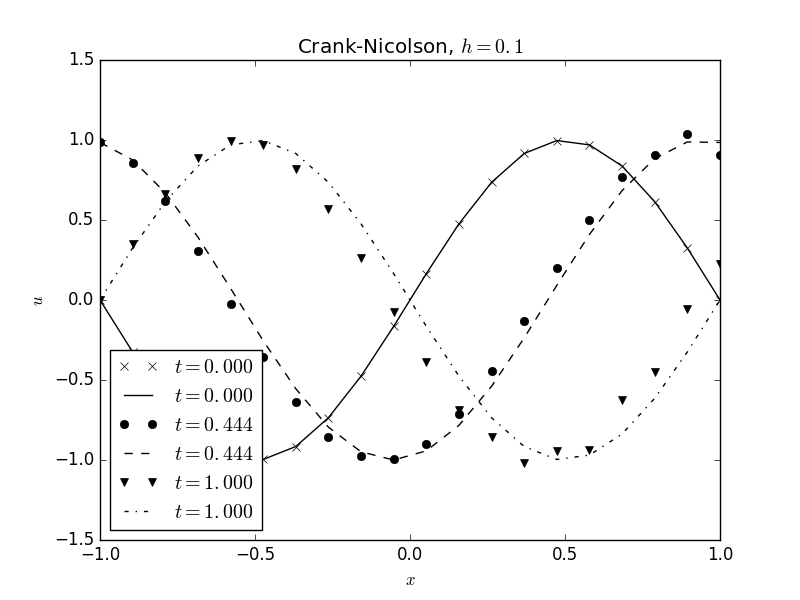
\includegraphics[width=\fw]{cn_thomas_M-20}
      \captionof{figure}{Crank-Nicolson scheme applied to the hyperbolic equation $u_t + u_x = 0$. The discretization is such that $h = \frac{1}{10}$ and $\lambda = 1.0$. The discrete solution (given by markers) is plotted with the exact solution (given by lines) for three different snapshots in time.}
      \vspace{0.25in}
      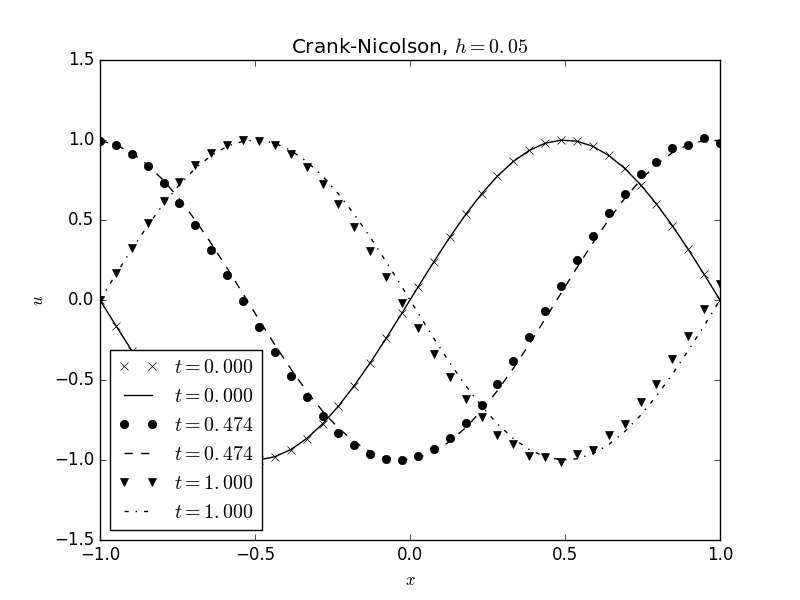
\includegraphics[width=\fw]{cn_thomas_M-40}
      \captionof{figure}{Crank-Nicolson scheme applied to the hyperbolic equation $u_t + u_x = 0$. The discretization is such that $h = \frac{1}{20}$ and $\lambda = 1.0$. The discrete solution (given by markers) is plotted with the exact solution (given by lines) for three different snapshots in time.}
      \vspace{0.25in}
      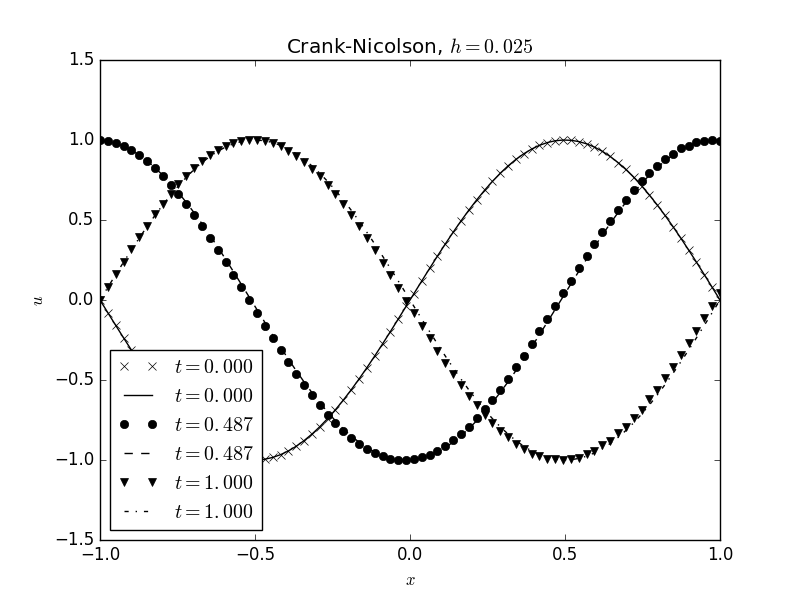
\includegraphics[width=\fw]{cn_thomas_M-80}
      \captionof{figure}{Crank-Nicolson scheme applied to the hyperbolic equation $u_t + u_x = 0$. The discretization is such that $h = \frac{1}{40}$ and $\lambda = 1.0$. The discrete solution (given by markers) is plotted with the exact solution (given by lines) for three different snapshots in time.}
      \vspace{0.25in}
    }
		
	\subsection{Source Code}
	
	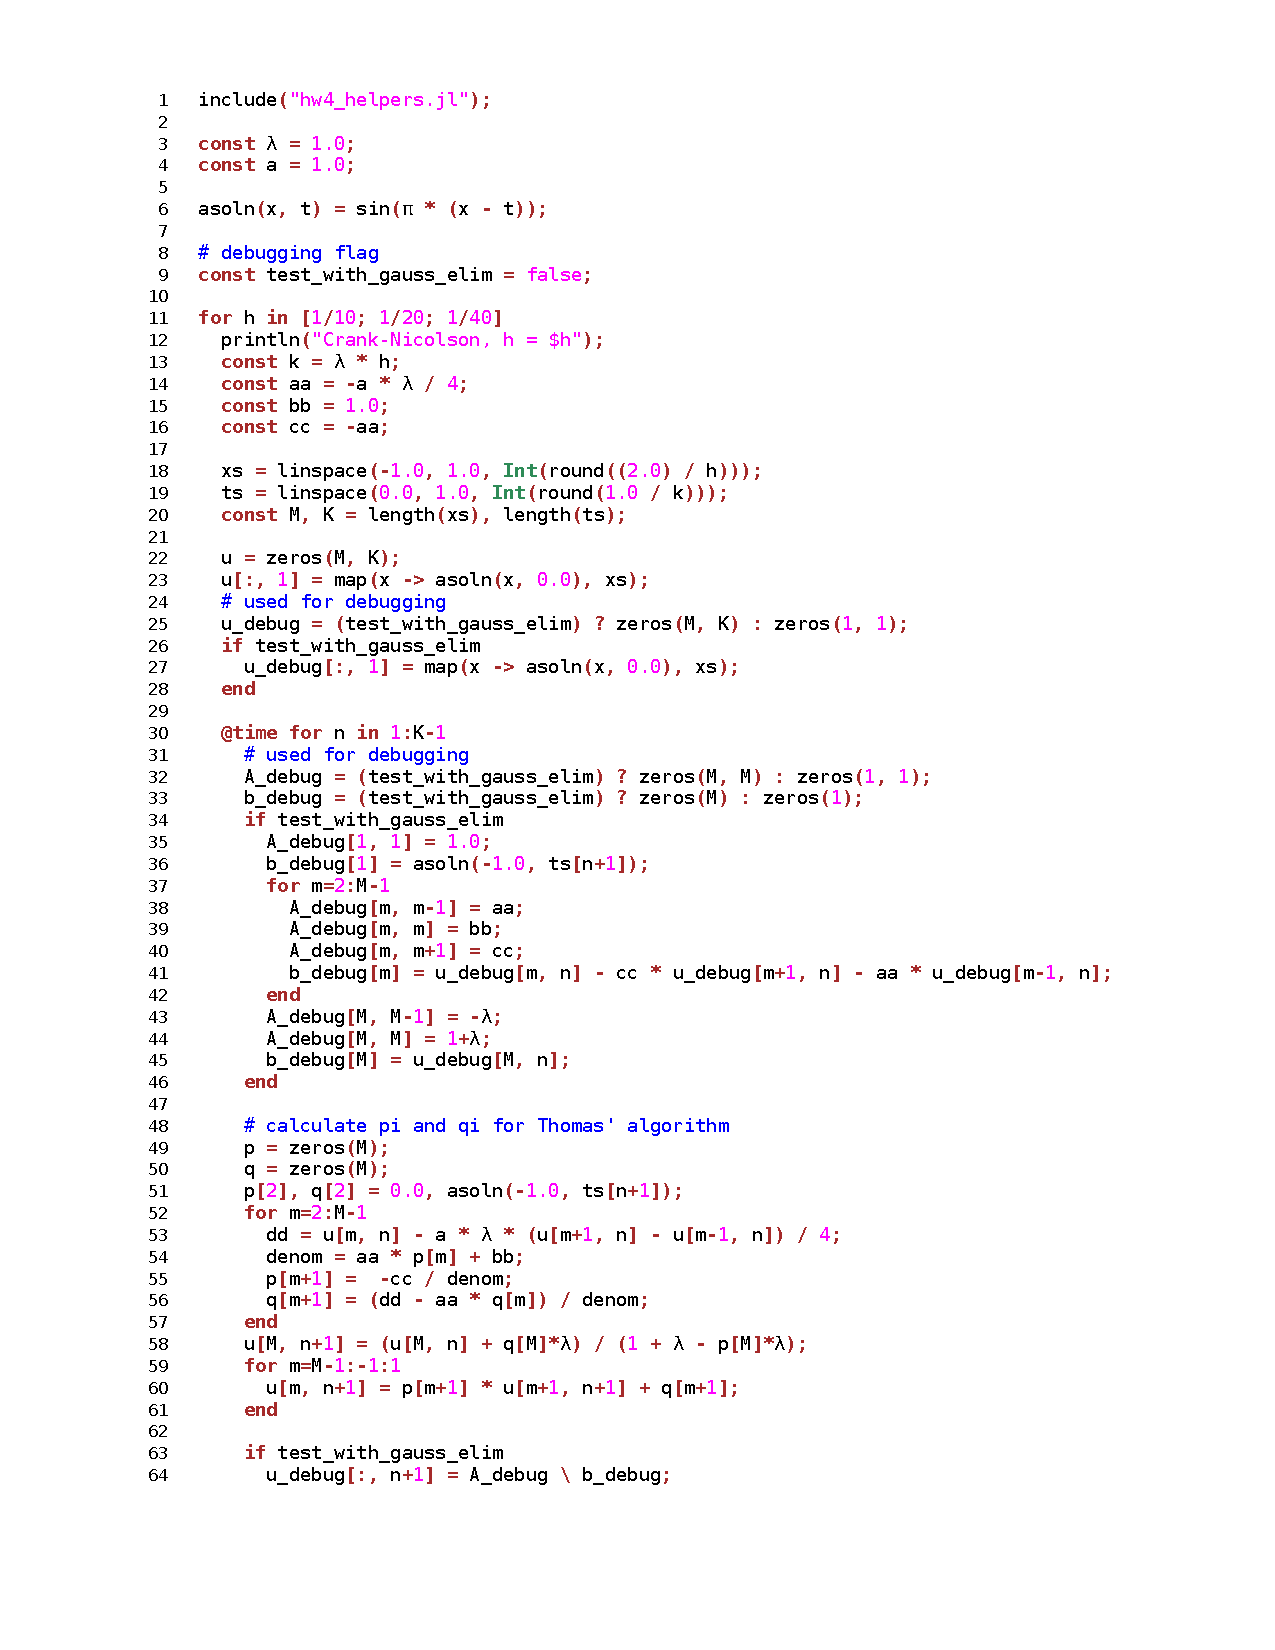
\includepdf[pages=-]{./hw4c1.pdf}
	
	\section{C2: Viscous Burgers' Equation} \label{sec:c2}
	
	\subsection{Constant $a$, $b$, and $c$. Varied $h$ and $k$.}
	
	In order to investigate the effect of grid spacing and time step size on the stability and accuracy of the forward time central space scheme applied to the viscous Burgers' equation, $a$, $b$, and $c$ were held constant while $h$ and $k$ were varied.
	In the first three figures $h = 0.1$ and $k$ is varied ($k = 0.001, 0.005$ and $0.01$).
	The discrete solution agrees well for $k = 0.001$ and $k = 0.005$.
	However, for $k = 0.01$ the discrete solution quickly diverges (becomes $NaN$ on the interior of the domain).
	
	The last figure is for $h = 0.2$ and $k = 0.01$.
	The stability of the solution in the figure shows that $k = 0.005$ is not some special time step size above which the solution diverges, but instead that the stability of the discrete solution is sensitive to the ratio between the time step size and the grid spacing.
	It appears as though the discrete solution becomes divergent when $\lambda > 0.05$ where $\lambda = \frac{k}{h}$.
	
	{
		\centering
		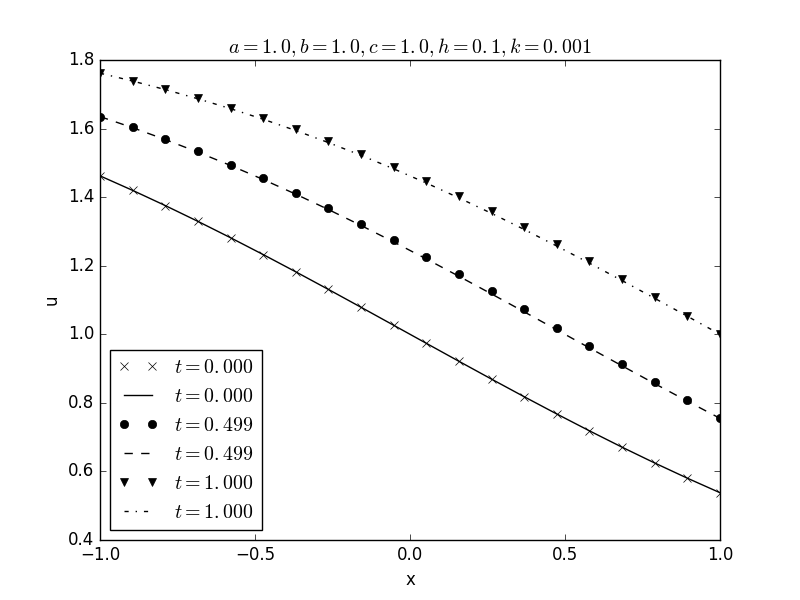
\includegraphics[width=\fw]{vb_a-100_b-100_c-100_h-0100_k-0001}
		\captionof{figure}{Forward time central space scheme applied to the viscous Burgers' equation $u_t + \left(\frac{u^2}{2}\right)_x = b u_{xx}$. The discrete solution (given by markers) is plotted with the exact solution, $u\left(x, t\right) = a - c \tanh \left(\frac{c}{2b}\left(x - at\right)\right)$ where $a = 1.0$, $b = 1.0$, $c = 1.0$, $h = 0.1$ and $k = 0.001$ (given by lines) for three different snapshots in time.}
		\vspace{0.25in}
		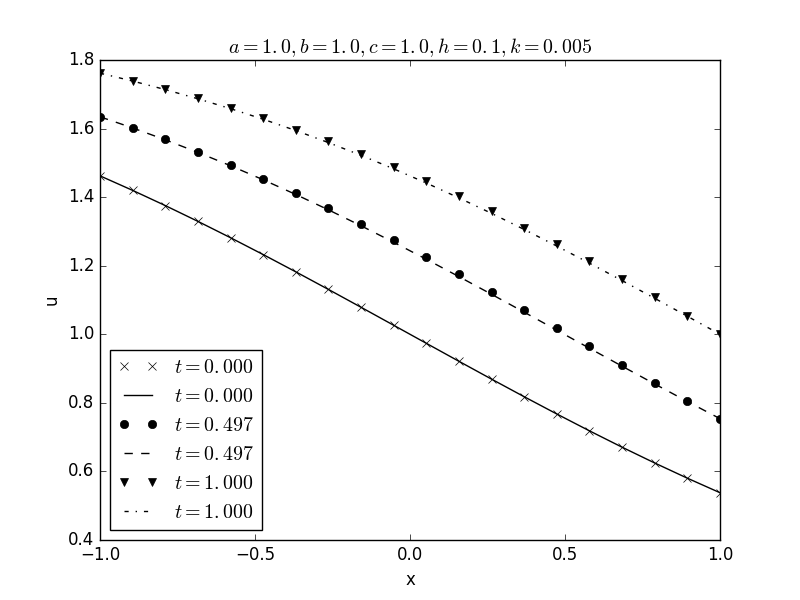
\includegraphics[width=\fw]{vb_a-100_b-100_c-100_h-0100_k-0005}
		\captionof{figure}{Forward time central space scheme applied to the viscous Burgers' equation $u_t + \left(\frac{u^2}{2}\right)_x = b u_{xx}$. The discrete solution (given by markers) is plotted with the exact solution, $u\left(x, t\right) = a - c \tanh \left(\frac{c}{2b}\left(x - at\right)\right)$ where $a = 1.0$, $b = 1.0$, $c = 1.0$, $h = 0.1$ and $k = 0.005$ (given by lines) for three different snapshots in time.}
		\vspace{0.25in}
		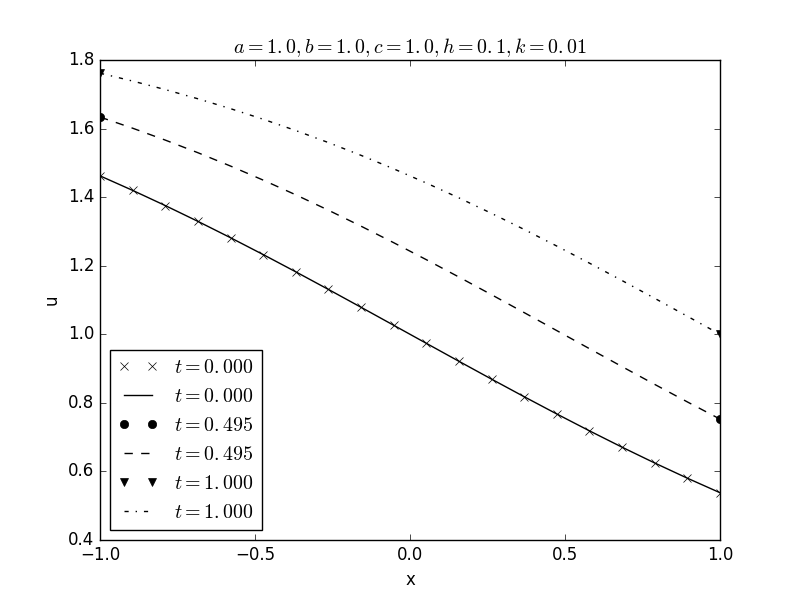
\includegraphics[width=\fw]{vb_a-100_b-100_c-100_h-0100_k-0010}
		\captionof{figure}{Forward time central space scheme applied to the viscous Burgers' equation $u_t + \left(\frac{u^2}{2}\right)_x = b u_{xx}$. The discrete solution (given by markers) is plotted with the exact solution, $u\left(x, t\right) = a - c \tanh \left(\frac{c}{2b}\left(x - at\right)\right)$ where $a = 1.0$, $b = 1.0$, $c = 1.0$, $h = 0.1$ and $k = 0.01$ (given by lines) for three different snapshots in time.}
		\vspace{0.25in}
		%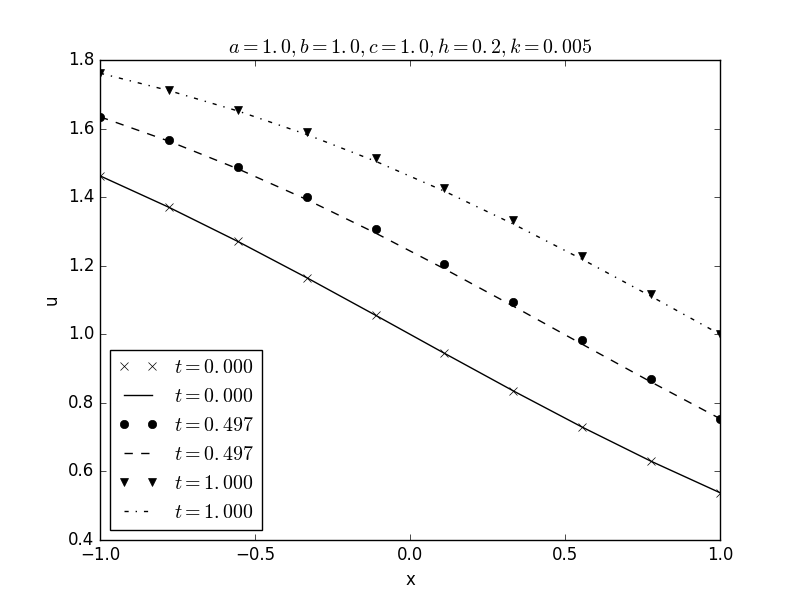
\includegraphics[width=\fw]{vb_a-100_b-100_c-100_h-0200_k-0005}
		%\captionof{figure}{Forward time central space scheme applied to the viscous Burgers' equation $u_t + \left(\frac{u^2}{2}\right)_x = b u_{xx}$. The discrete solution (given by markers) is plotted with the exact solution, $u\left(x, t\right) = a - c \tanh \left(\frac{c}{2b}\left(x - at\right)\right)$ where $a = 1.0$, $b = 1.0$, $c = 1.0$, $h = 0.2$ and $k = 0.005$ (given by lines) for three different snapshots in time.}
		%\vspace{0.25in}
		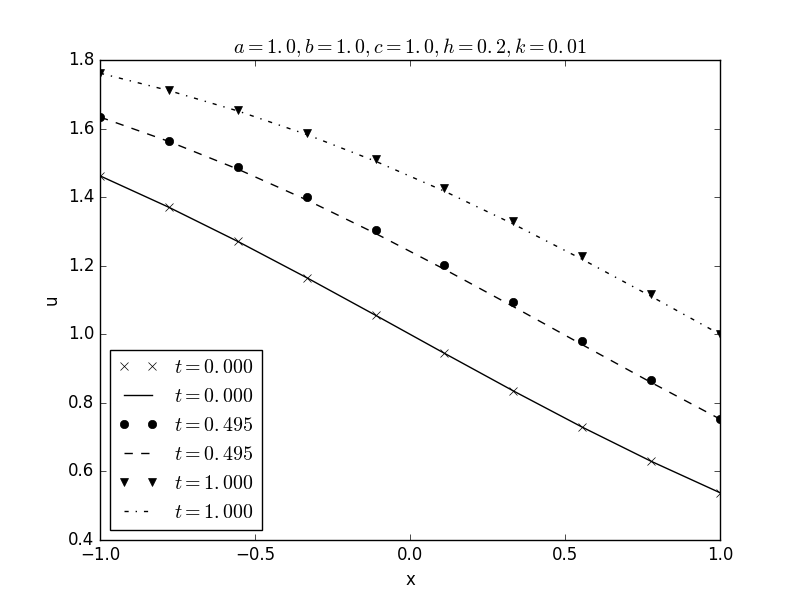
\includegraphics[width=\fw]{vb_a-100_b-100_c-100_h-0200_k-0010}
		\captionof{figure}{Forward time central space scheme applied to the viscous Burgers' equation $u_t + \left(\frac{u^2}{2}\right)_x = b u_{xx}$. The discrete solution (given by markers) is plotted with the exact solution, $u\left(x, t\right) = a - c \tanh \left(\frac{c}{2b}\left(x - at\right)\right)$ where $a = 1.0$, $b = 1.0$, $c = 1.0$, $h = 0.2$ and $k = 0.01$ (given by lines) for three different snapshots in time.}
		\vspace{0.25in}
	}
	
	\subsection{Constant $a$, $c$, $h$ and $k$. Varied $b$.}
	
	In order to investigate the effect of the diffusion coefficient on the stability and accuracy of the forward time central space scheme applied to the viscous Burgers' equation, $a$, $c$, $h$ and $k$ were held constant while $b$ was varied; $b = 0.5, 0.1, 0.01, 0.001$.
	As $b$ is decreased, the solution becomes more nonlinear.
	For $b = 0.5$ and $0.1$ the discrete solution agrees well with the exact solution.
	However, for smaller values of $b$ ($b = 0.01, 0.001$) large oscillations manifest in the discrete solution.
	
	{
		\centering
		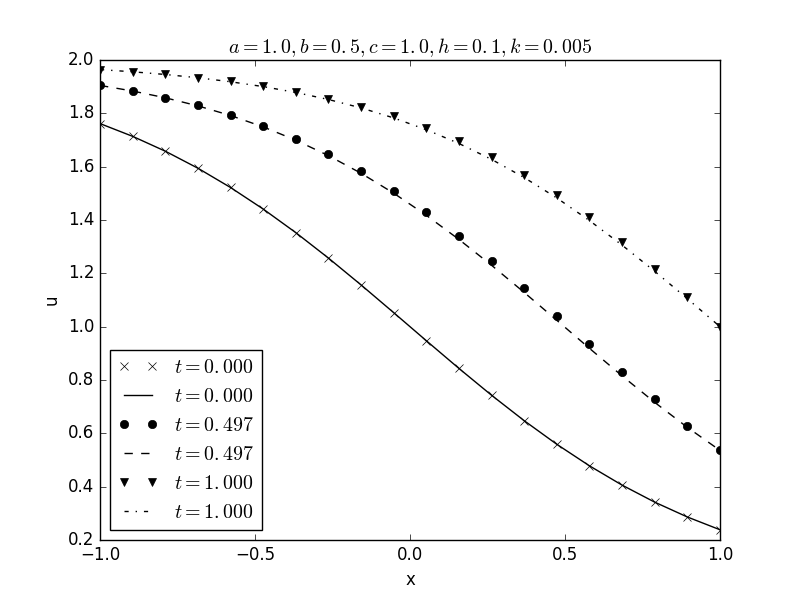
\includegraphics[width=\fw]{vb_a-100_b-050_c-100_h-0100_k-0005}
		\captionof{figure}{Forward time central space scheme applied to the viscous Burgers' equation $u_t + \left(\frac{u^2}{2}\right)_x = b u_{xx}$. The discrete solution (given by markers) is plotted with the exact solution, $u\left(x, t\right) = a - c \tanh \left(\frac{c}{2b}\left(x - at\right)\right)$ where $a = 1.0$, $b = 0.5$, $c = 1.0$, $h = 0.1$ and $k = 0.005$ (given by lines) for three different snapshots in time.}
		\vspace{0.25in}
		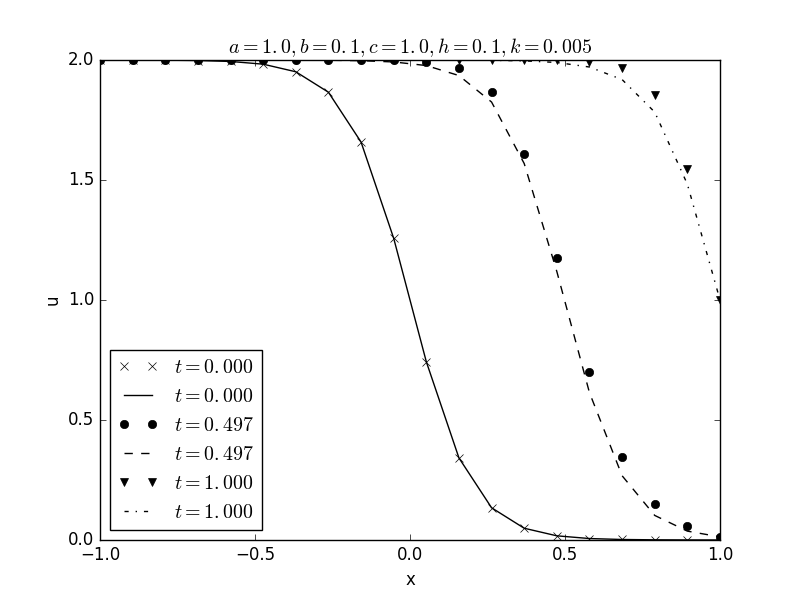
\includegraphics[width=\fw]{vb_a-100_b-010_c-100_h-0100_k-0005}
		\captionof{figure}{Forward time central space scheme applied to the viscous Burgers' equation $u_t + \left(\frac{u^2}{2}\right)_x = b u_{xx}$. The discrete solution (given by markers) is plotted with the exact solution, $u\left(x, t\right) = a - c \tanh \left(\frac{c}{2b}\left(x - at\right)\right)$ where $a = 1.0$, $b = 0.1$, $c = 1.0$, $h = 0.1$ and $k = 0.005$ (given by lines) for three different snapshots in time.}
		\vspace{0.25in}
		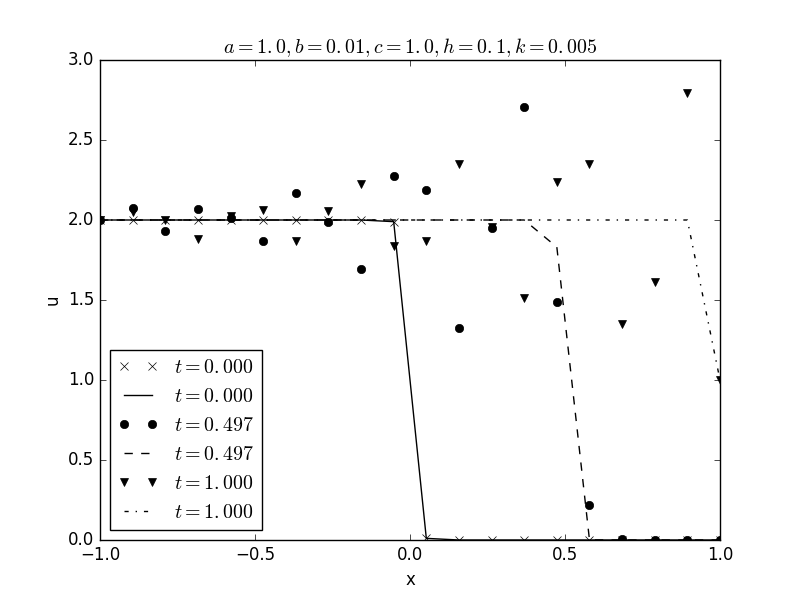
\includegraphics[width=\fw]{vb_a-100_b-001_c-100_h-0100_k-0005}
		\captionof{figure}{Forward time central space scheme applied to the viscous Burgers' equation $u_t + \left(\frac{u^2}{2}\right)_x = b u_{xx}$. The discrete solution (given by markers) is plotted with the exact solution, $u\left(x, t\right) = a - c \tanh \left(\frac{c}{2b}\left(x - at\right)\right)$ where $a = 1.0$, $b = 0.01$, $c = 1.0$, $h = 0.1$ and $k = 0.005$ (given by lines) for three different snapshots in time.}
		\vspace{0.25in}
		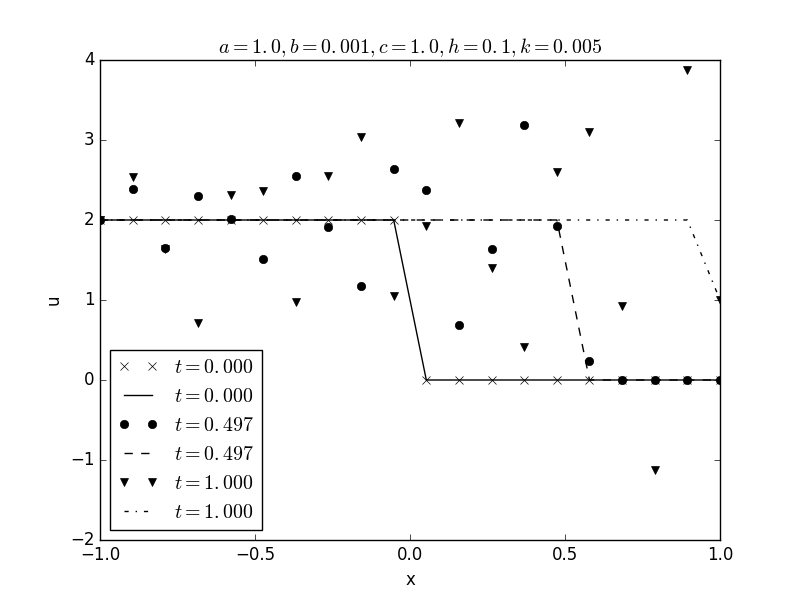
\includegraphics[width=\fw]{vb_a-100_b-000_c-100_h-0100_k-0005}
		\captionof{figure}{Forward time central space scheme applied to the viscous Burgers' equation $u_t + \left(\frac{u^2}{2}\right)_x = b u_{xx}$. The discrete solution (given by markers) is plotted with the exact solution, $u\left(x, t\right) = a - c \tanh \left(\frac{c}{2b}\left(x - at\right)\right)$ where $a = 1.0$, $b = 0.001$, $c = 1.0$, $h = 0.1$ and $k = 0.005$ (given by lines) for three different snapshots in time.}
		\vspace{0.25in}
	}
	
	\subsection{Source Code}
	
	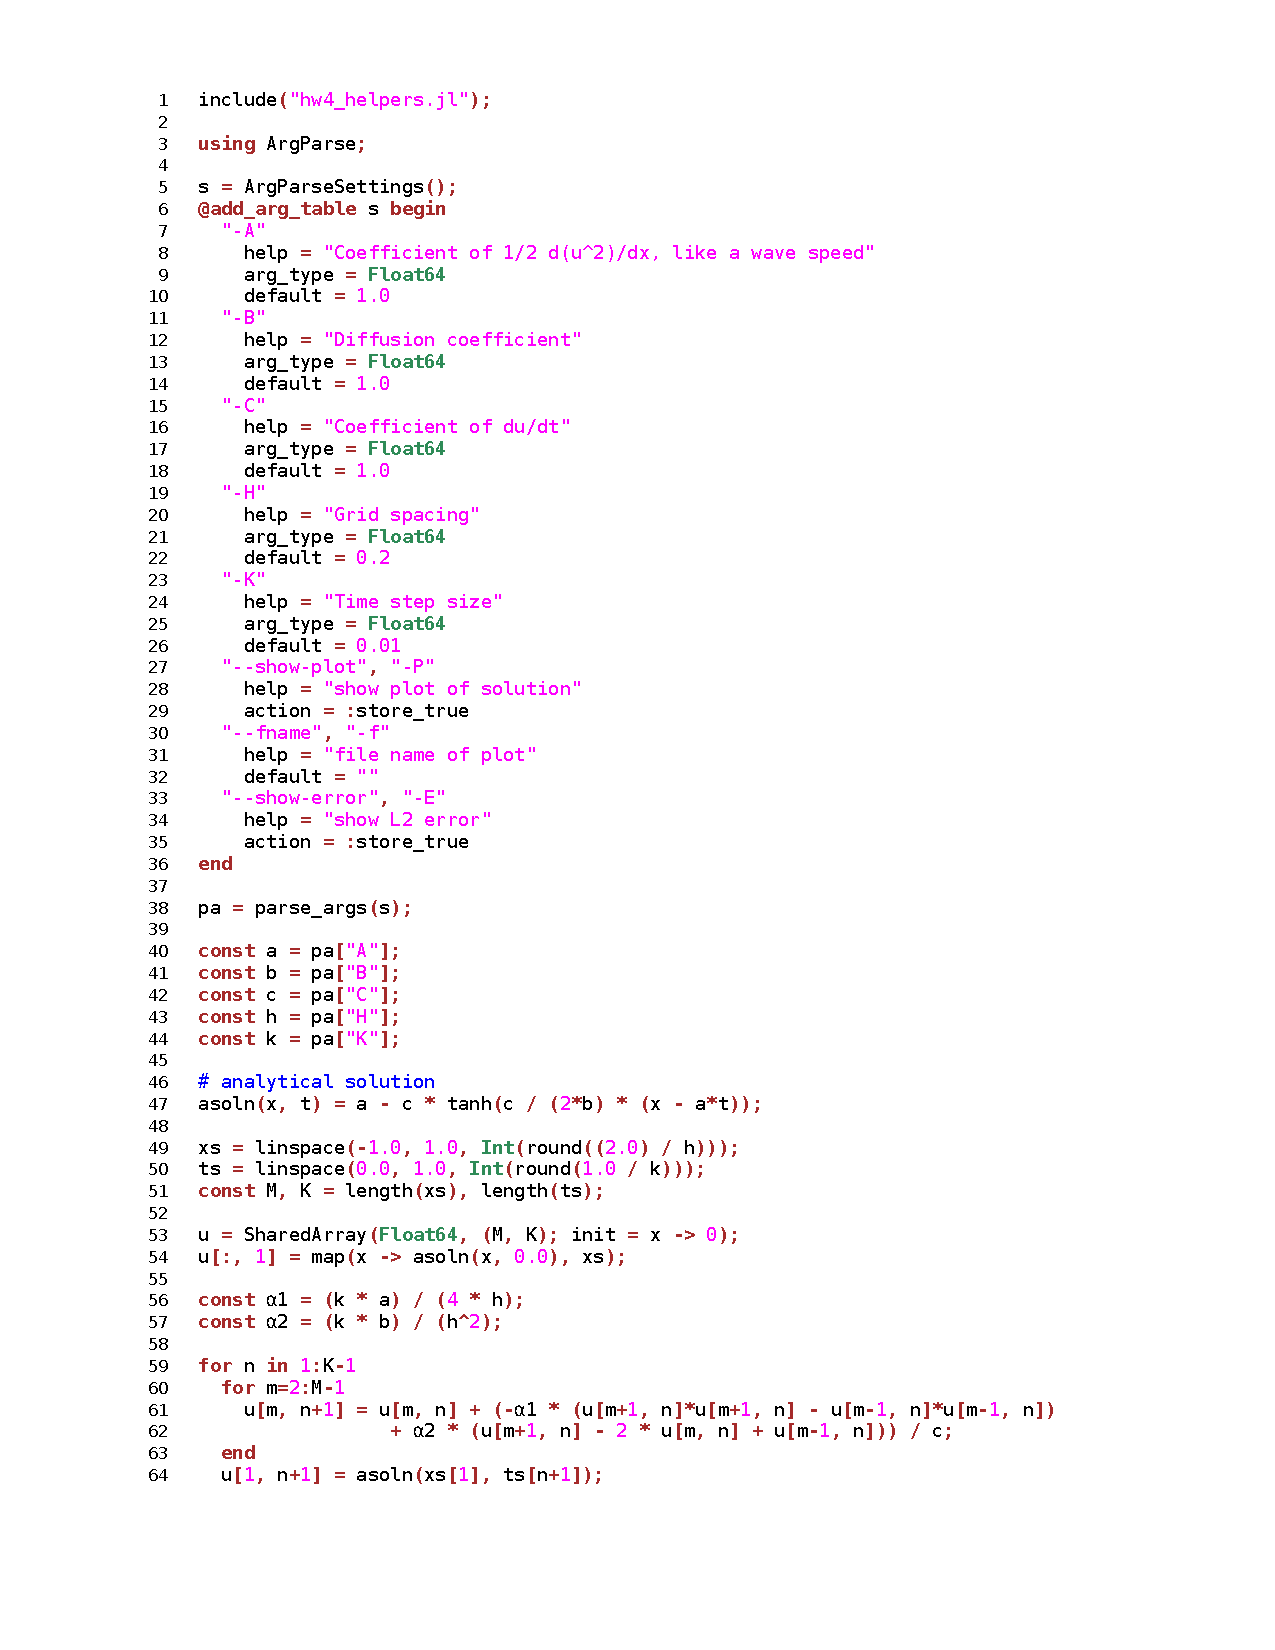
\includepdf[pages=-]{./hw4c2.pdf}
	
	\section{Shared Code}
	
	Some visualization code was shared between the files for \Fref{sec:c1} and \Fref{sec:c2}.
	For the sake of completeness, it is included below.
	
	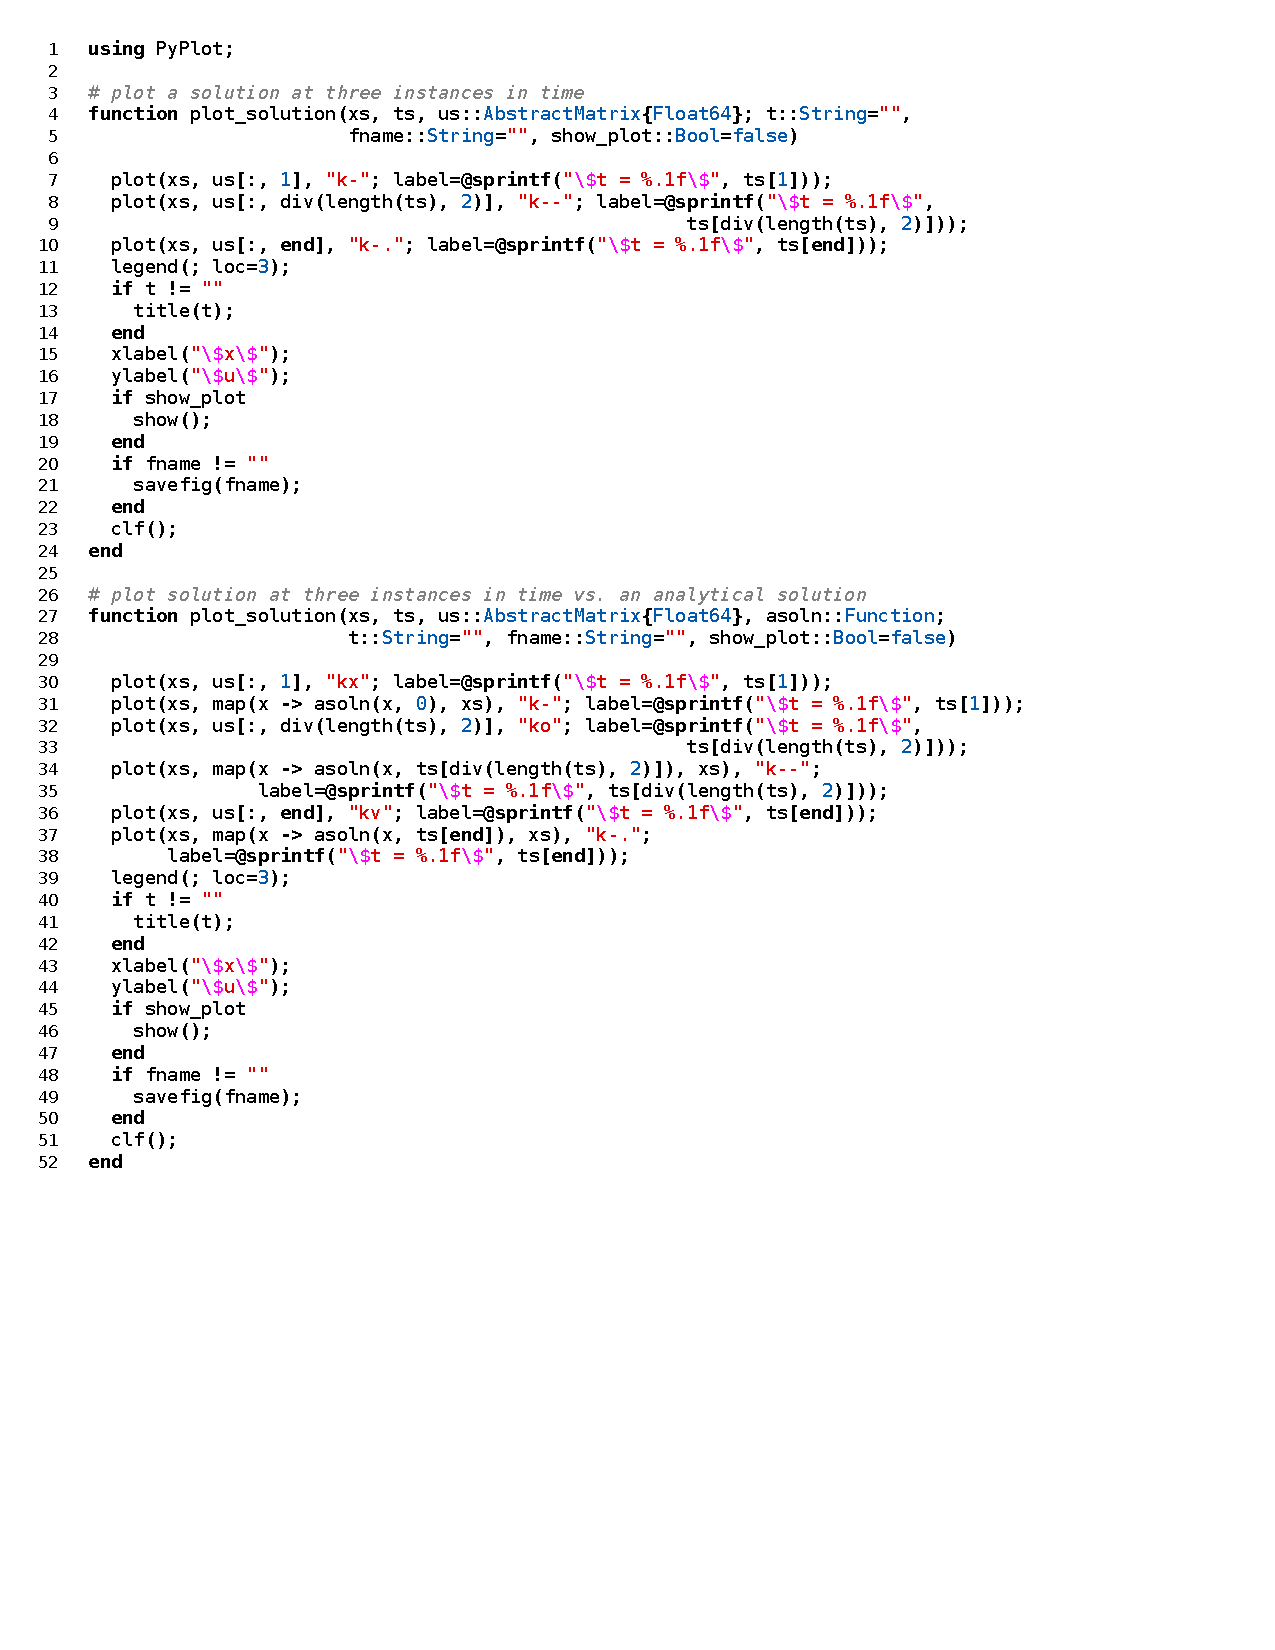
\includepdf[pages=-]{./hw4_helpers.pdf}
	
\end{document}
